\section{Χάρτης}
Ακριβώς από κάτω από την μπάρα αναζήτησης βρίσκεται στα αριστερά ένας παγκόσμιος χάρτης ο οποίος έχει δεδομένα για όλες τις χώρες οι οποίες έχουν παράξει έστω και μια ταινία και βρίσκονται φυσικά στην βάση δεδομένων της εφαρμογής.
Οι χώρες στον χάρτη χρωματίζονται από διαφορετικές αποχρώσεις του μπλε, όσο πιο έντονο είναι το χρώμα τόσες παραπάνω ταινίες έχει αυτή η χώρα. Ο Χάρτης υποστηρίζει μεγέθυνσή και κύλιση. Αν ο χρήστης μετακινήσει τον κένσορα του ποντικιού πάνω από μια χώρα ένα βοηθητικό παραθυράκι θα εμφανιστεί από πάνω αναγράφοντας το όνομα της χώρα και το πόσες ταινίες έχει όπως φαίνεται στη εικόνα \ref{demo:map}. Ο χρωματισμός και τα δεδομένα του χάρτη παραμένουν τα ίδια ανεξάρτητα απο την κατηγορία ή το έτος που έχει επιλεγεί.

\begin{figure}[H]
  \centering
  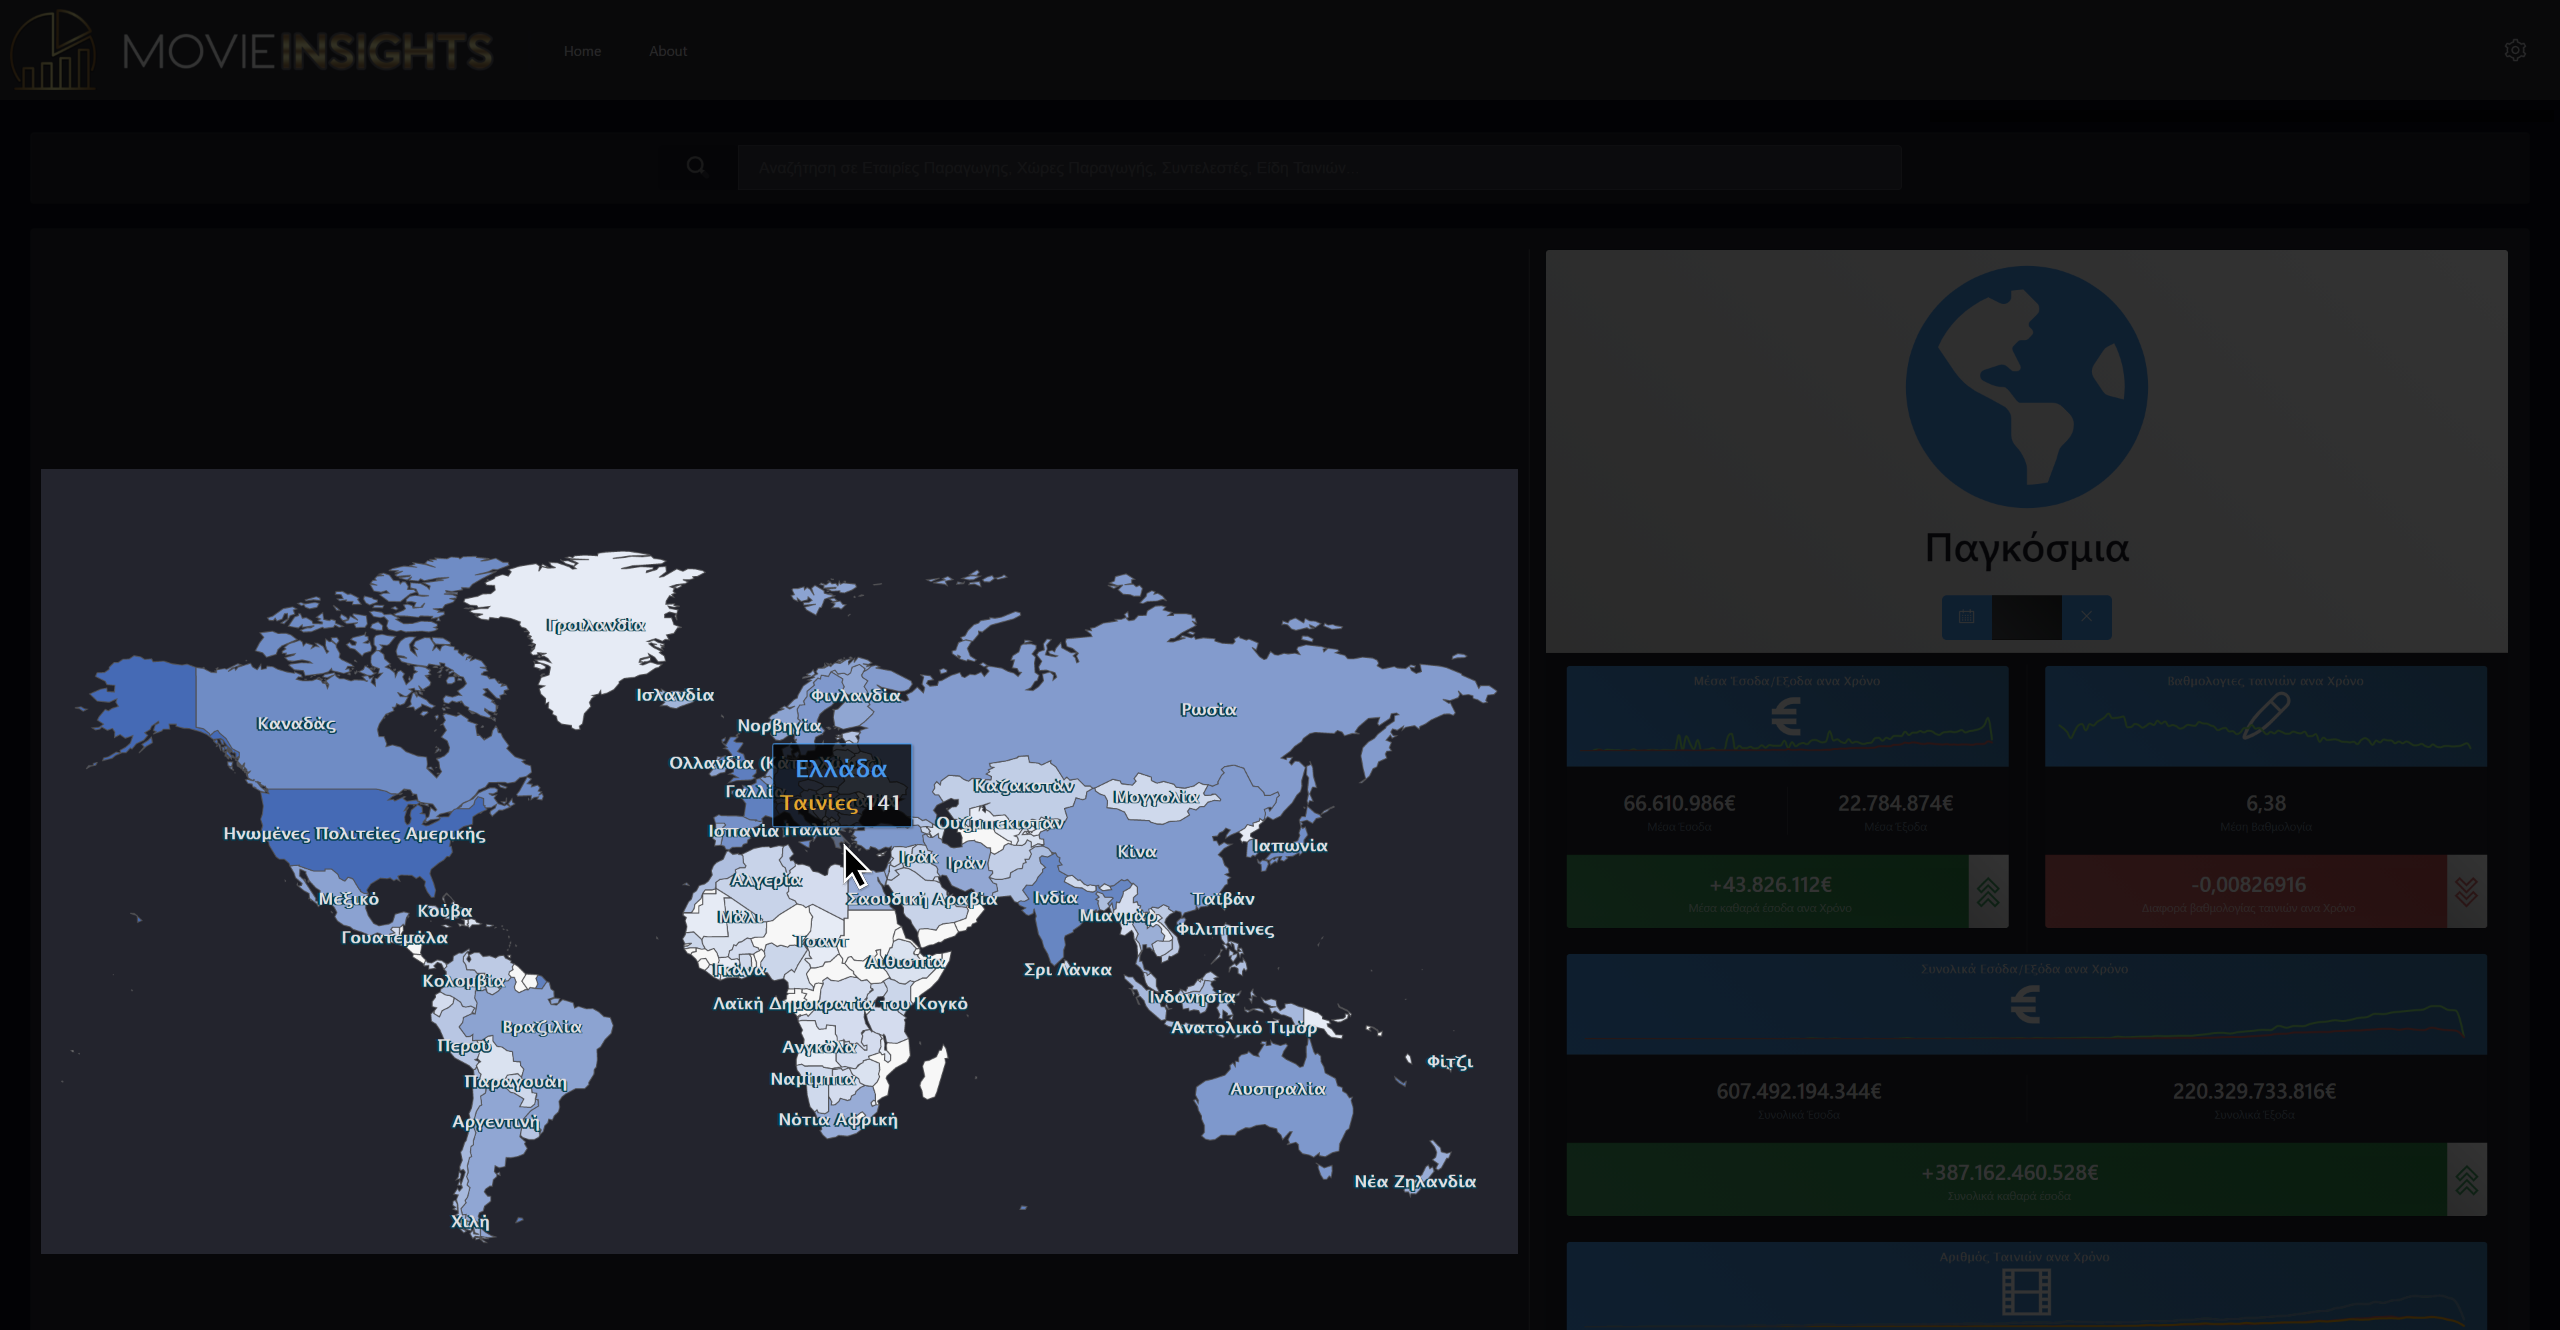
\includegraphics[width=145mm]{Chapters/6 - Manual/Images/main_page_map.png}
  \caption{Παγκόσμιος Χάρτης}
  \label{demo:map}
\end{figure}